\documentclass[fleqn]{jbook}
\usepackage{physpub}
% amsmath, graphicx は自動的に読み込まれるので
% \usepackage しないでください、してもかまわないけど。
\begin{document}

\begin{question}{第2問}{佐々井健蔵}
図のように$N$個の単量体が連結された直線的な鎖状分子を考える。各単量体は図のように自由に変形し、
長さ$a$の状態$\alpha $(エネルギー:$+\epsilon $)か長さ$b$の状態$\beta $(エネルギー:$-\epsilon $)のいずれかを、
隣り合う単量体とは独立にとることができるとする。
% 図の挿入
\begin{figure}[htbp]
  \begin{center}
    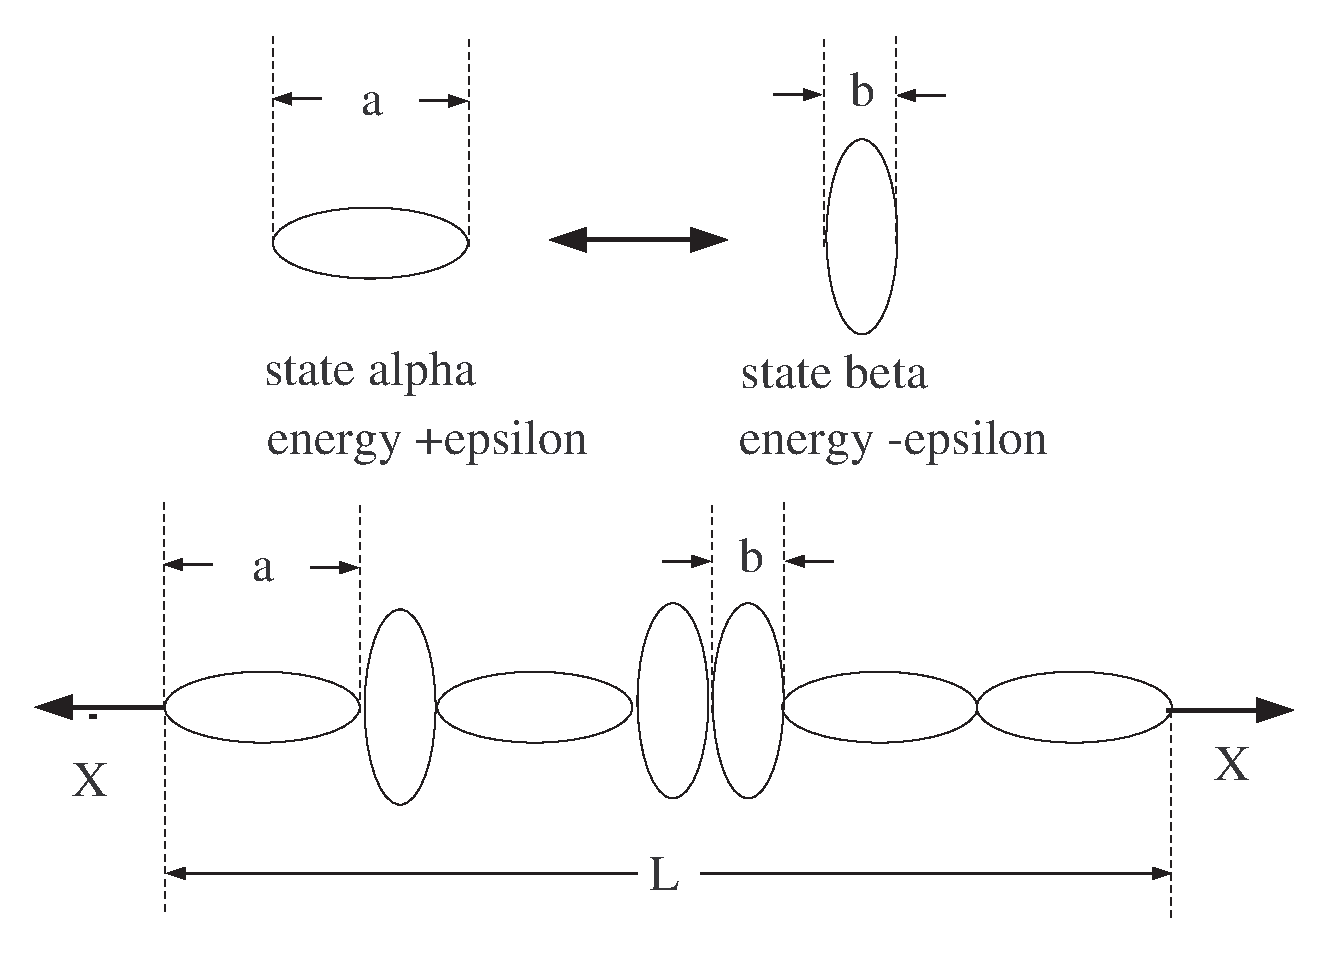
\includegraphics[keepaspectratio=true,height=60mm]{2003phy2-1.eps}
  \end{center}
  \caption{}%{}内にタイトルを記入してください
\end{figure}

鎖状分子が独立した状態にあって、熱平衡に達している場合(ミクロカノニカル分布)を考える。
\begin{enumerate}
\item $N_{\alpha }$個が$\alpha $、$N_{\beta }$個が$\beta $の状態にいる場合を考える($N=N_{\alpha }+N_{\beta }$)。
鎖状分子の長さ$L$とエネルギー$E_{L}$を求めよ。また、この状態の熱力学的重率$W(N_{\alpha },N_{\beta })$を求め、
鎖状分子のエントロピー$S$が次のようになることを示せ。
\begin{equation}
S=-k_B\left\{N_{\alpha }\log \frac{N_{\alpha }}{N}+N_{\beta }\log \frac{N_{\beta }}{N}\right\}
\end{equation}
ここで$k_B$はボルツマン定数である。Stirlingの公式、$\log n!=n\log n-n(n\gg 1)$を用いてよい。また、$\log $は自然対数とする。
\end{enumerate}

つぎに、鎖状分子が温度$T$の熱浴に接していて、一定の温度状態におかれている場合(カノニカル分布)を考える。
\begin{enumerate}
\setcounter{enumi}{1}
\item 熱浴の状態密度を$\Omega (E_B)$とする。鎖状分子と熱浴からなる全系のエネルギーを$E_T$、状態$l$にある鎖状分子のエネルギーを$E_l$とすれば
($E_T=E_B+E_l$)、等重率の原理により、状態$l$の実現確率は$P(E_l)$は、$l$が指定された場合の微視的状態の数$\Omega (E_T-E_l)\delta E$に比例する。
\begin{equation}
P(E_l)\propto \frac{\Omega (E_T-E_l)\delta E}{\Omega (E_T)\delta E}
\end{equation}
このことから、カノニカル分布では、状態$l$の実現状態$P(E_l)$は、$\exp (-E_l/k_BT)$に比例することを示せ。
ただし、熱浴は鎖状分子に比べて十分大きいものとする。また、熱浴の温度が
$T=(\partial S/\partial E)^{-1}|_{E=E_T}$で表せることに留意せよ。
\item 一つの単量体の分配関数$Z_1$を示し、さらに鎖状分子の分配関数$Z_N$を導け。
\item 分配関数$Z_N$より、Helmholtzの自由エネルギー$F$、エントロピー$S$、系の内部エネルギー$E$を求めよ。
\item 比熱$C$を求め、温度の関数として図示せよ。ただし縦軸を$C/Nk_B$とし、横軸を$k_BT/\epsilon $とせよ。
\end{enumerate}

つぎに、鎖状分子を温度$T$の状態においたまま、一定の張力$X$で両端を引っ張り、長さ$L$となった場合を考える。
このとき、この系では、熱力学第一法則$TdS=dE-XdL$が成立している。($N$個の単量体からなる系を、
非常に大きな$N_T$個からなる非常に大きな系と考えることが出来る。)
\begin{enumerate}
\setcounter{enumi}{5}
\item 鎖状分子がエネルギー$E_L$で長さ$L$の状態にある確率$p(E_L,L)$は、熱浴を含む全系のエネルギーを$E_T$、
長さを$L_T$とすると、熱浴の状態密度$\Omega (E_B)=\Omega (E_T-E_L,L_T-L)$を用いて
\begin{equation}
p(E_L,L)\propto \frac{\Omega (E_T-E_L,L_T-L)\delta E}{\Omega (E_T,L_T)\delta E}
\end{equation}
と書ける。$E_T$、$L_T$に比べて、$E_L$、$L$が十分微視的な料であることを利用して、
\begin{equation}
p(E_L,L)\propto \exp \left\{\ \frac{1}{k_BT} (-E_L+XL)\right\}
\end{equation}
であることを示せ。

\item 系の分配関数
\begin{equation}
Y=\sum ^{N}_{N_{\alpha }=0}W(N_{\alpha },N_{\beta })p(E(N_{\alpha },N_{\beta }),L(N_{\alpha },N_{\beta }))
\end{equation}
について、$N_{\alpha }$に関する和を計算し、$N,T,X,a,b,+\epsilon ,-\epsilon $を用いて表せ。
\item 分配関数よりGibbsの自由エネルギー$G$を求め、そこから鎖状分子の長さ$L$と張力$X$に関する関係式を求めよ。
\end{enumerate}
\end{question}

\begin{answer}{第2問}{佐々井健蔵}
\begin{enumerate}
\item 熱力学的重率とは、指定された値に対して可能な量子状態数であるので
\begin{equation}
W(N_{\alpha },N_{\beta })=\frac{N!}{N_{\alpha }!N_{\beta }!}
\end{equation}

\item エントロピー$S$は、Stirlingの公式を用いて、
\begin{equation}
S=k_B\log W=k_B[N\log N-(N_{\alpha }\log N_{\alpha })-(N_{\beta }\log N_{\beta })]
=-k_B\left( N_{\alpha }\log \frac{N_{\alpha }}{N}+N_{\beta }\log \frac{N_{\beta }}{N}\right)
\end{equation}

\item $\delta E$が小さい場合、
\begin{equation}
\Omega (E)\delta E=W
\end{equation}
となるので、
\begin{equation}
p(E_l)\propto \exp \left[ \frac{S(E_T-E_l)-S(E_T)}{k_B}\right]
\end{equation}
熱浴は十分大きいので$E_T\gg E_l$、これをふまえて$S(E_T-E_l)-S(E_T)$を展開すると、
\begin{equation}
S(E_T-E_l)-S(E_T)=-E_l\left.\frac{\partial S}{\partial E}\right|_{E=E_T}
                    +\frac{1}{2}E_l^2\left.\frac{\partial ^2S}{\partial E^2}\right|_{E=E_T}+\cdots 
\end{equation}
オーダーで考えれば、第二項以降は第一項に$E_l/E_T$をかけたものと同程度の大きさしかなく、
第一項に比べて無視できるので、$T=(\partial S/\partial E)^{-1}|_{E=E_T}$も用いて
\begin{equation}
P(E_l)\propto \exp (-E_l/k_BT)
\end{equation}

\item $\beta =1/k_BT$として、
\begin{equation}
Z_1=e^{-\beta \epsilon }+e^{\beta \epsilon }=2\cosh \beta \epsilon
\end{equation}
\begin{equation}
Z_N=Z_1^N=(2\cosh \beta \epsilon)^N
\end{equation}

\item 
\begin{equation}
F=-k_BT\log Z_N=-Nk_BT \log (2\cosh \beta \epsilon)
\end{equation}
\begin{equation}
S=-\frac{\partial F}{\partial T}=Nk_B\left[ \log (2\cosh \beta \epsilon)-\frac{\epsilon }{k_BT}\tanh \beta \epsilon \right]
\end{equation}
\begin{equation}
E=F+TS=-N \epsilon \tanh \beta \epsilon
\end{equation}
\item
\begin{equation}
C=\frac{\partial E}{\partial T}=Nk_B(\beta \epsilon)^2 \frac{1} {\cosh ^2\beta \epsilon}
\end{equation}
関数形は$y=C/Nk_B,x=k_BT/\epsilon $として
\begin{equation}
y=\frac{1}{x^2\cosh ^2(\frac{1}{x})}
\end{equation}
% 図の挿入
\begin{figure}[htbp]
  \begin{center}
    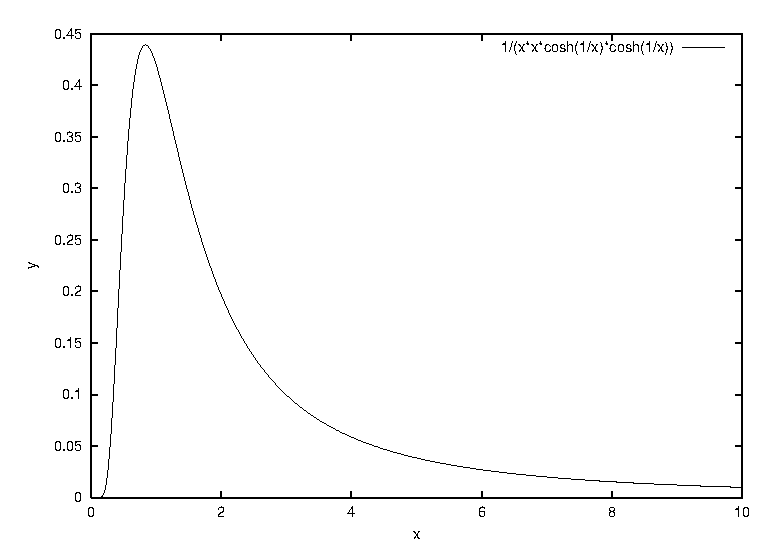
\includegraphics[keepaspectratio=true,height=100mm]{2003phy2-2.eps}
  \end{center}
  \caption{}%{}内にタイトルを記入してください
\end{figure}
\item 2番と同様に
\begin{equation}
p(E_L,L) \propto \exp \left[ \frac{S(E_T-E_L,L_T-L)-S(E_T,L_T)}{k_B}\right]
\end{equation}
$E_T\gg E_L,L_T\gg L$より$S(E_T-E_L,L_T-L)-S(E_T,L_T)$を展開すると、
\begin{align*}
S(E_T-E_L,L_T-L)&-S(E_T,L_T)=-E_L\left. \frac{\partial S}{\partial E}\right|_{E=E_T}
                            -L  \left. \frac{\partial S}{\partial L}\right|_{L=L_T}\\
&+\frac{1}{2}\left( E_L^2\left. \frac{\partial ^2S}{\partial E^2}\right|_{E=E_T} 
+2E_L L \left. \frac{\partial ^2S}{\partial E \partial L}\right|_{E=E_T,L=L_T}
+L^2  \left. \frac{\partial ^2 S}{\partial L^2}\right|_{L=L_T}\right)+\cdots
\end{align*}
オーダーで考えると、第二項以降は第一項に$E_L/ E_T,L/L_T$をかけたもの程度の大きさしかなく、
第一項に比べて無視できるので、$T=(\partial S/\partial E)^{-1}|_{E=E_T}$と$TdS=dE-XdL$も用いると、
\begin{equation}
S(E_T-E_L,L_T-L)-S(E_T,L_T)=\frac{-E_L+XL}{T}
\end{equation}
\begin{equation}
\therefore p(E_L,L)\propto \exp \left\{\ \frac{1}{k_BT} (-E_L+XL)\right\}
\end{equation}

\item $L(N_{\alpha },N_{\beta })=N_{\alpha }a+N_{\beta }b,
E_L(N_{\alpha },N_{\beta })=N_{\alpha }\epsilon -N_{\beta }\epsilon$と、
二項定理$\sum_{k=0}^{n}\binom{n}{k}a^{n-k}b^{k}=(a+b)^n$を用いて、
\begin{align*}
Y&=\sum ^{N}_{N_{\alpha}=0}\frac{N!}{N_{\alpha }!N_{\beta }!}e^{ \beta (-E_L+XL) }\\
 &=\sum ^{N}_{N_{\alpha}=0}\frac{N!}{N_{\alpha }!(N-N_{\alpha })!}
   \left[e^{\beta (aX-\epsilon )}\right]^{N_{\alpha }}
   \left[e^{\beta (bX+\epsilon )}\right]^{N-N_{\alpha }}\\
 &=\left[e^{\beta (aX-\epsilon )}+e^{\beta (bX+\epsilon )}\right]^N
\end{align*}
\item \begin{equation}
G=-k_BT\log Y =-Nk_BT\log \left[e^{\beta (aX-\epsilon )}+e^{\beta (bX+\epsilon )}\right]
\end{equation}
また、$G=F-XL,dG=-SdT-LdX$より、
\begin{equation}
L=-\frac{\partial G}{\partial X}
=\frac{N\left[ae^{\beta (aX-\epsilon )}+be^{\beta (bX+\epsilon )}\right]}
{e^{\beta (aX-\epsilon )}+e^{\beta (bX+\epsilon )}}
\end{equation}

\end{enumerate}
\end{answer}


\end{document}
